% ============================================================
% TAREFA 9 — VAR ou VEC? Análise Dinâmica na Cadeia do Diesel
% PPGE / FURG | Econometria
% Compilar com: xelatex -interaction=nonstopmode tarefa9.tex (2×)
% ============================================================
\documentclass[12pt,a4paper]{article}

% ── Codificação e fontes ───────────────────────────────────
\usepackage{fontspec}
\setmainfont{Times New Roman}
\usepackage[portuguese]{babel}

% ── Layout ────────────────────────────────────────────────
\usepackage[top=2.5cm, bottom=2.5cm, left=3cm, right=2.5cm]{geometry}
\setlength{\headheight}{14pt}
\usepackage{setspace}
\onehalfspacing

% ── Matemática ────────────────────────────────────────────
\usepackage{amsmath, amssymb, mathtools}

% ── Tabelas e figuras ─────────────────────────────────────
\usepackage{booktabs, multirow, array, longtable}
\usepackage{graphicx}
\usepackage{float}
\usepackage{caption}
\captionsetup{font=small, labelfont=bf}

% ── Código R ──────────────────────────────────────────────
\usepackage{xcolor}
\usepackage{listings}

\definecolor{codebg}{RGB}{248,248,248}
\definecolor{codecomment}{RGB}{100,100,100}
\definecolor{codekeyword}{RGB}{0,0,180}
\definecolor{codestring}{RGB}{0,128,0}

\lstdefinestyle{Rstyle}{
  language=R,
  backgroundcolor=\color{codebg},
  commentstyle=\color{codecomment}\itshape,
  keywordstyle=\color{codekeyword}\bfseries,
  stringstyle=\color{codestring},
  basicstyle=\ttfamily\footnotesize,
  breaklines=true,
  frame=single,
  framerule=0.4pt,
  rulecolor=\color{gray!50},
  tabsize=2,
  showstringspaces=false,
  captionpos=b,
  numbers=none
}
\lstset{style=Rstyle}

% ── Cabeçalho/rodapé ──────────────────────────────────────
\usepackage{fancyhdr}
\pagestyle{fancy}
\fancyhf{}
\fancyhead[L]{\small PPGE -- FURG $|$ Econometria}
\fancyhead[R]{\small Tarefa 9}
\fancyfoot[C]{\thepage}
\renewcommand{\headrulewidth}{0.4pt}

% ── Hyperlinks (carregado depois de listings para evitar conflito) ─────────
\usepackage[colorlinks=true, linkcolor=blue!70!black, citecolor=blue!70!black]{hyperref}

% ── Formatação de seções ──────────────────────────────────
\usepackage{titlesec}
\titleformat{\section}{\large\bfseries}{\thesection}{1em}{}[\vspace{-0.3em}\rule{\linewidth}{0.4pt}]
\titleformat{\subsection}{\normalsize\bfseries}{\thesubsection}{1em}{}

% ────────────────────────────────────────────────────────────────────
\begin{document}

% ── Página de título ─────────────────────────────────────
\thispagestyle{empty}
\begin{center}
  {\large\bfseries UNIVERSIDADE FEDERAL DO RIO GRANDE -- FURG}\\[0.3em]
  {\normalsize Instituto de Ciências Econômicas, Administrativas e Contábeis}\\
  {\normalsize Programa de Pós-Graduação em Economia Aplicada}
\end{center}

\vspace{3.5cm}
\begin{center}
  \rule{\linewidth}{0.6pt}\\[0.6em]
  {\LARGE\bfseries Tarefa 9}\\[0.4em]
  {\large VAR ou VEC? Especificação, Estimação e Análise Dinâmica}\\[0.2em]
  {\large\itshape na Cadeia do Diesel --- Brasil (2023--2026)}\\[0.4em]
  \rule{\linewidth}{0.6pt}
\end{center}

\vspace{3cm}
\begin{center}
  Disciplina: Econometria\\[0.4em]
  Discente: Arthur Pereira Donato\\[0.2em]
  Matrícula: 184210\\[0.2em]
  Professor: Cristiano Aguiar de Oliveira
\end{center}

\vspace{4cm}
\begin{center}
  Rio Grande, 22 de junho de 2026
\end{center}

\newpage

% ── Sumário ─────────────────────────────────────────────
\tableofcontents
\newpage

% ============================================================
\section{Parte 1 -- Preparação e Análise Exploratória}
% ============================================================

A base utilizada é a série semanal de preços de combustíveis da ANP,
com 161 observações entre 02/01/2023 e 26/01/2026.
As três variáveis de interesse são o Brent em reais por barril
(\texttt{brent\_brl\_media}), o preço do Diesel A~S10 na refinaria/produtor
(\texttt{dieselA\_S10\_pi}) e o preço do Diesel B~S10 na distribuidora
(\texttt{dieselB\_S10\_dist}).
Todas foram transformadas em logaritmo natural, de modo que diferenças
de log aproximam taxas de variação e coeficientes de regressão
correspondem a elasticidades.

\subsection{Item 1 -- Carregamento, Truncamento e Estatísticas Descritivas}

\begin{lstlisting}[caption={Carregamento, truncamento e criação das variáveis em log}]
# Carrega a base ANP e aplica o truncamento em 26/01/2026
dados <- read.csv("dados_diesel.csv", stringsAsFactors = FALSE, sep = ",")
dados$data_inicio <- as.Date(dados$data_inicio)
dados <- dados[dados$data_inicio <= as.Date("2026-01-26"), ]  # 161 obs.

# Logaritmos naturais das tres series de interesse
dados$l_brent <- log(dados$brent_brl_media)   # Brent R$/barril
dados$l_dA    <- log(dados$dieselA_S10_pi)    # Diesel A S10, produtor
dados$l_dB    <- log(dados$dieselB_S10_dist)  # Diesel B S10, distribuidor
\end{lstlisting}

\begin{table}[H]
\centering
\caption{Estatísticas Descritivas das Séries em Logaritmo Natural ($T = 161$)}
\label{tab:desc}
\begin{tabular}{lrrrrrrr}
\toprule
Variável & Média & D.P. & Mín. & Q1 & Mediana & Q3 & Máx. \\
\midrule
$\ln(\text{Brent})$ & 6,0094 & 0,0958 & 5,8071 & 5,9258 & 6,0261 & 6,0762 & 6,2183 \\
$\ln(\text{Diesel A})$ & 1,3415 & 0,0777 & 1,1132 & 1,3112 & 1,3573 & 1,3730 & 1,5129 \\
$\ln(\text{Diesel B})$ & 1,6605 & 0,0623 & 1,4694 & 1,6474 & 1,6763 & 1,6893 & 1,7570 \\
\bottomrule
\end{tabular}
\end{table}

\noindent
As estatísticas da Tabela~\ref{tab:desc} revelam que o Diesel B situa-se
sistematicamente acima do Diesel A (mediana 1,676 vs.\ 1,357 em log),
diferença que reflete a margem de distribuição e a tributação adicional
incorporada ao ponto de venda.
A dispersão relativa do Brent (D.P.\ $= 0,096$) é maior do que a do
Diesel A (0,078) e do Diesel B (0,062), compatível com a suavização
que a política de preços e os contratos de distribuição introduzem
ao longo da cadeia.

\subsection{Item 2 -- Séries em Log ao Longo do Tempo}

\begin{lstlisting}[caption={Painel de séries em log ao longo do tempo (fig01)}]
png("outputs/fig01_series_log.png", width = 900, height = 720)
par(mfrow = c(3, 1), mar = c(3, 4, 2.5, 1))

plot(dados$data_inicio, dados$l_brent, type = "l", col = "steelblue", lwd = 1.5,
     xlab = "Data", ylab = "log(R$/barril)",
     main = "l_brent - Brent em R$/barril (log natural)")
abline(h = mean(dados$l_brent), lty = 2, col = "gray40")
legend("topright", c("Serie", "Media"), lty = c(1,2),
       col = c("steelblue","gray40"), bty = "n", cex = 0.85)

plot(dados$data_inicio, dados$l_dA, type = "l", col = "darkorange", lwd = 1.5,
     xlab = "Data", ylab = "log(R$/litro)",
     main = "l_dA - Diesel A S10, Produtor (log natural)")
abline(h = mean(dados$l_dA), lty = 2, col = "gray40")

plot(dados$data_inicio, dados$l_dB, type = "l", col = "darkgreen", lwd = 1.5,
     xlab = "Data", ylab = "log(R$/litro)",
     main = "l_dB - Diesel B S10, Distribuidor (log natural)")
abline(h = mean(dados$l_dB), lty = 2, col = "gray40")
dev.off()
\end{lstlisting}

\begin{figure}[H]
  \centering
  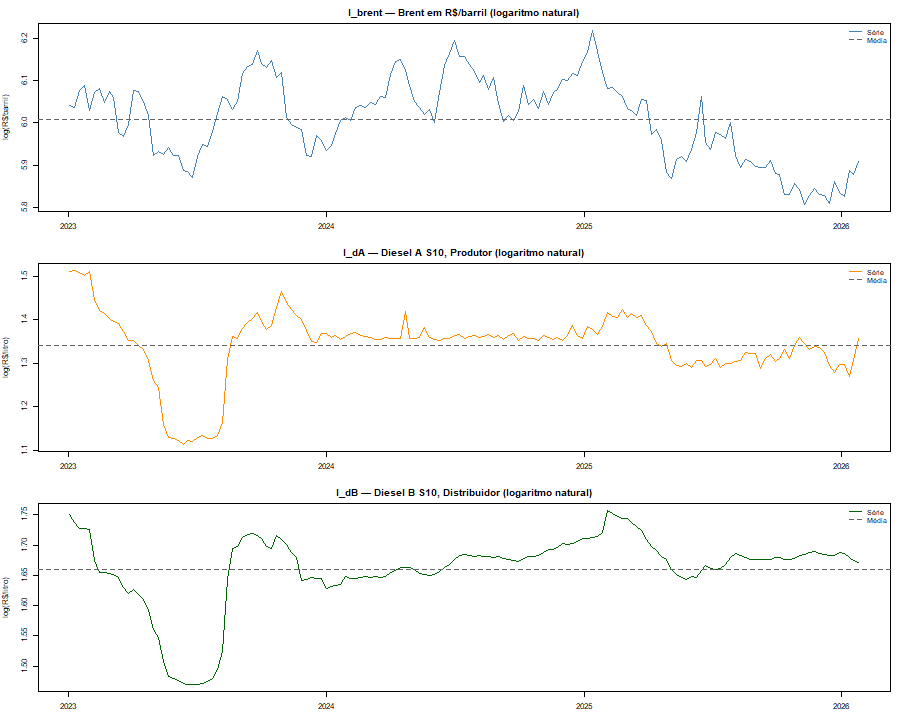
\includegraphics[width=\linewidth]{outputs/fig01_series_log.png}
  \caption{Séries em logaritmo natural (2023--2026).
           A linha tracejada indica a média amostral de cada série.}
  \label{fig:series}
\end{figure}

\noindent
Os três gráficos da Figura~\ref{fig:series} sugerem a presença de
\textbf{tendência estocástica}: nenhuma das séries oscila em torno de
um nível fixo; ao contrário, exibem deriva persistente e desvios
prolongados em relação à média.
O \textbf{co-movimento} entre as três séries é visível, em especial a
queda simultânea no primeiro semestre de 2023 e a posterior
recuperação, indício de que compartilham um componente de longo
prazo --- motivação para o teste de cointegração.

\subsection{Item 3 -- Correlogramas ACF}

\begin{lstlisting}[caption={ACF em nível e em primeira diferença (fig02 e fig03)}]
# ACF em nivel: decaimento lento indica raiz unitaria I(1)
png("outputs/fig02_acf_nivel.png", width = 900, height = 720)
par(mfrow = c(3, 1), mar = c(3, 4, 2.5, 1))
acf(dados$l_brent, lag.max = 20, main = "ACF - l_brent (nivel)")
acf(dados$l_dA,    lag.max = 20, main = "ACF - l_dA (nivel)")
acf(dados$l_dB,    lag.max = 20, main = "ACF - l_dB (nivel)")
dev.off()

# ACF em 1a diferenca: colapso imediato confirma I(1) -> diferenca I(0)
png("outputs/fig03_acf_diff.png", width = 900, height = 720)
par(mfrow = c(3, 1), mar = c(3, 4, 2.5, 1))
acf(diff(dados$l_brent), lag.max = 20, main = "ACF - Dl_brent (1a diferenca)")
acf(diff(dados$l_dA),    lag.max = 20, main = "ACF - Dl_dA (1a diferenca)")
acf(diff(dados$l_dB),    lag.max = 20, main = "ACF - Dl_dB (1a diferenca)")
dev.off()
\end{lstlisting}

\begin{figure}[H]
  \centering
  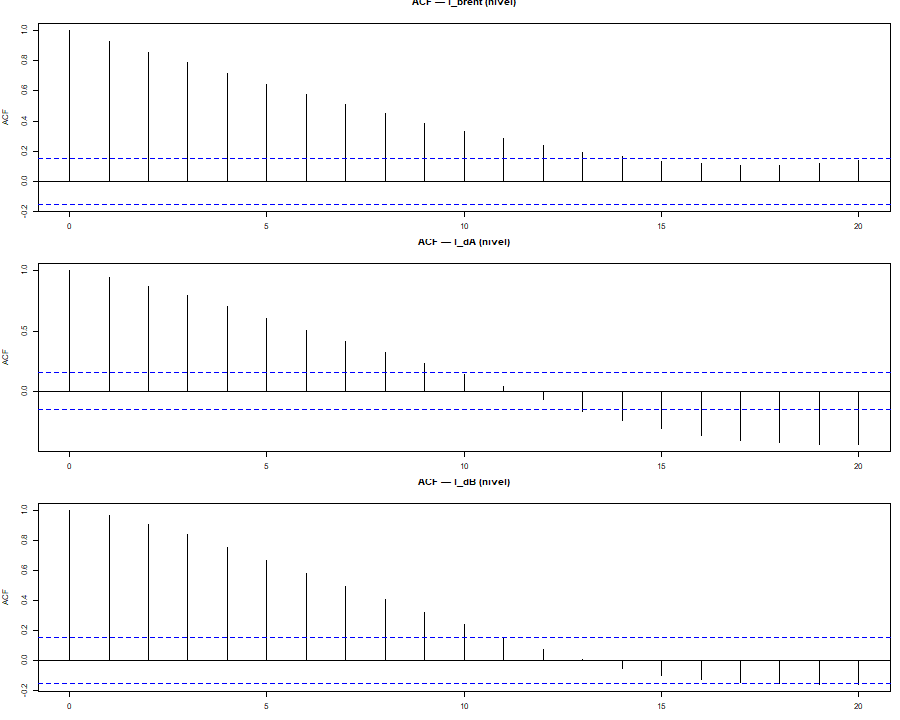
\includegraphics[width=\linewidth]{outputs/fig02_acf_nivel.png}
  \caption{ACF em nível (até defasagem 20). Decaimento lento, típico de séries I(1).}
  \label{fig:acf_nivel}
\end{figure}

\begin{figure}[H]
  \centering
  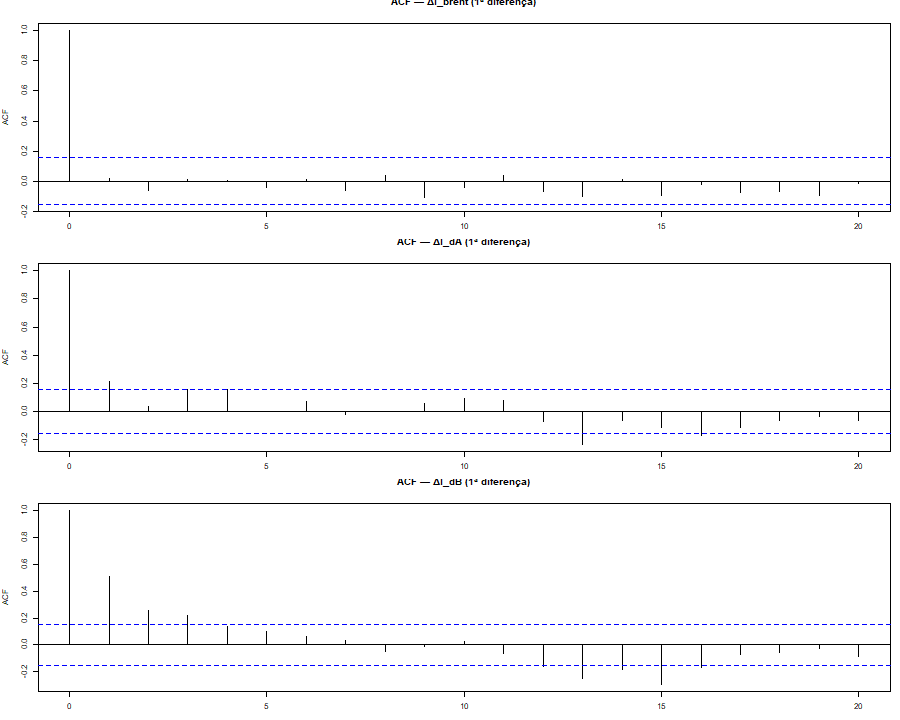
\includegraphics[width=\linewidth]{outputs/fig03_acf_diff.png}
  \caption{ACF em primeira diferença. Colapso imediato ao intervalo de confiança.}
  \label{fig:acf_diff}
\end{figure}

\noindent
A ACF em nível (Figura~\ref{fig:acf_nivel}) apresenta autocorrelações
próximas de 1 que decaem de forma extremamente lenta --- padrão clássico
de série integrada de ordem 1.
Após a diferenciação (Figura~\ref{fig:acf_diff}), as autocorrelações
colapsam imediatamente para dentro do intervalo de confiança de $\pm 1{,}96/\sqrt{T}$,
comportamento consistente com série $I(0)$ (ruído branco).
O padrão em dois estágios é \textbf{consistente com a hipótese $I(1)$}
para as três variáveis.

% ============================================================
\section{Parte 2 -- Testes de Raiz Unitária}
% ============================================================

\subsection{Item 4 -- Teste ADF}

\begin{lstlisting}[caption={ADF com type="none", lags=6, selectlags="AIC" (pacote urca)}]
# H0: raiz unitaria. Rejeita se tau < -1,95 (CV 5%, tau_nc, T~160)
adf_teste <- function(serie) {
  res <- ur.df(serie, type = "none", lags = 6, selectlags = "AIC")
  tau <- res@teststat[1]    # estatistica de teste
  res                       # retorna objeto completo
}

# Nivel
adf_brent <- adf_teste(dados$l_brent)
adf_dA    <- adf_teste(dados$l_dA)
adf_dB    <- adf_teste(dados$l_dB)

# Primeira diferenca
adf_Dbrent <- adf_teste(diff(dados$l_brent))
adf_DdA    <- adf_teste(diff(dados$l_dA))
adf_DdB    <- adf_teste(diff(dados$l_dB))
\end{lstlisting}

\begin{table}[H]
\centering
\caption{Resultados dos Testes ADF (type = "none"; CV 5\% $= -1{,}95$)}
\label{tab:adf}
\begin{tabular}{llrrl}
\toprule
Série & Ordem & $\hat{\tau}$ & CV 5\% & Decisão \\
\midrule
$\ell\_\text{brent}$ & nível & $-0{,}421$ & $-1{,}95$ & Raiz unitária \\
$\ell\_dA$           & nível & $-0{,}254$ & $-1{,}95$ & Raiz unitária \\
$\ell\_dB$           & nível & $\phantom{-}0{,}026$ & $-1{,}95$ & Raiz unitária \\
\midrule
$\Delta\ell\_\text{brent}$ & 1ª dif. & $-8{,}923$ & $-1{,}95$ & Estacionária \\
$\Delta\ell\_dA$           & 1ª dif. & $-5{,}545$ & $-1{,}95$ & Estacionária \\
$\Delta\ell\_dB$           & 1ª dif. & $-5{,}973$ & $-1{,}95$ & Estacionária \\
\bottomrule
\end{tabular}
\end{table}

\noindent
Em nível, nenhuma das três séries rejeita a hipótese nula de raiz unitária
(os valores $|\hat{\tau}|$ ficam bem abaixo de 1,95).
Em primeira diferença, todas rejeitam de forma robusta ($|\hat{\tau}| > 5$,
muito acima até do valor crítico de 1\%: $-2{,}58$).
\textbf{As três séries são $I(1)$}, condição necessária para a aplicação do
modelo VEC.

\subsection{Item 5 -- Especificação: VAR em Diferenças, VAR em Níveis ou VEC?}

Como as três séries são $I(1)$, há três especificações possíveis:
(i)~\textbf{VAR em diferenças}: correto se não houver cointegração ($r=0$),
mas descarta a informação de longo prazo;
(ii)~\textbf{VAR em níveis}: geraria regressão espúria para $I(1)$ sem cointegração;
(iii)~\textbf{VEC}: especificação eficiente se $1 \le r < k$, pois incorpora
tanto a dinâmica de curto prazo quanto o mecanismo de correção de erros (ECT).
A \textbf{condição necessária para o VEC} é que as séries sejam $I(1)$ e
que exista ao menos uma combinação linear estacionária entre elas ($r \ge 1$).
A decisão entre essas alternativas é determinada pelo teste de Johansen (Parte~4).

% ============================================================
\section{Parte 3 -- Seleção da Ordem do Modelo}
% ============================================================

\subsection{Item 6 -- VARselect}

\begin{lstlisting}[caption={VARselect para p = 1,...,8 com type="none"}]
Y <- cbind(l_brent = dados$l_brent,
           l_dA    = dados$l_dA,
           l_dB    = dados$l_dB)

sel <- VARselect(Y, lag.max = 8, type = "none")
print(round(sel$criteria, 4))
\end{lstlisting}

\begin{table}[H]
\centering
\caption{Critérios de Seleção de Defasagens (VARselect, $p = 1$ a $8$)}
\label{tab:varsel}
\resizebox{\linewidth}{!}{%
\begin{tabular}{lrrrrrrrr}
\toprule
Critério & $p=1$ & $p=2$ & $p=3$ & $p=4$ & $p=5$ & $p=6$ & $p=7$ & $p=8$ \\
\midrule
AIC & $-23{,}572$ & $\mathbf{-23{,}856}$ & $-23{,}835$ & $-23{,}795$ & $-23{,}724$ & $-23{,}680$ & $-23{,}619$ & $-23{,}567$ \\
HQ  & $-23{,}500$ & $\mathbf{-23{,}712}$ & $-23{,}618$ & $-23{,}505$ & $-23{,}362$ & $-23{,}246$ & $-23{,}112$ & $-22{,}988$ \\
SC  & $-23{,}394$ & $\mathbf{-23{,}500}$ & $-23{,}300$ & $-23{,}082$ & $-22{,}833$ & $-22{,}611$ & $-22{,}372$ & $-22{,}141$ \\
FPE & \multicolumn{8}{c}{$5{,}79 \times 10^{-11}$ a $5{,}87 \times 10^{-11}$ (mínimo em $p=2$)} \\
\bottomrule
\end{tabular}}
\end{table}

\noindent
Todos os quatro critérios (AIC, HQ, SC/BIC e FPE) elegem unanimemente $p = 2$.

\subsection{Item 7 -- Justificativa da Ordem $p = 2$}

Com $k = 3$ variáveis e $T = 161$, cada defasagem adicional consome
$k^2 = 9$ parâmetros (3 equações $\times$ 3 variáveis), reduzindo os graus
de liberdade e aumentando o risco de overfitting.
A escolha $p = 2$ é parcimoniosa e captura a autocorrelação relevante de
curto prazo, como confirmado pelos critérios: o AIC cai de $-23{,}572$
(em $p=1$) para $-23{,}856$ (em $p=2$) e volta a subir a partir de $p=3$.
No VECM, a ordem de defasagens nas diferenças será $p - 1 = 1$, resultado
em um modelo com $1 + 3 \times 1 = 4$ regressores por equação além do ECT
--- gerenciável dado o tamanho amostral.

% ============================================================
\section{Parte 4 -- Teste de Cointegração de Johansen}
% ============================================================

\subsection{Item 8 -- Estatísticas do Traço e do Máximo Autovalor}

\begin{lstlisting}[caption={Teste de Johansen com ca.jo() — ecdet="none", K=2}]
# ecdet="none": sem constante no vetor de cointegracao (consistente com ADF)
# K=2: correspondente a p=2 no VAR (K-1=1 lag de diferencas no VECM)
# spec="longrun": parametrizacao em forma de longo prazo
jo_trace <- ca.jo(Y, type = "trace", ecdet = "none", K = 2, spec = "longrun")
jo_eigen <- ca.jo(Y, type = "eigen", ecdet = "none", K = 2, spec = "longrun")
\end{lstlisting}

\begin{table}[H]
\centering
\caption{Teste de Johansen --- Estatísticas e Valores Críticos ($k=3$, $T=161$)}
\label{tab:johansen}
\resizebox{\linewidth}{!}{%
\begin{tabular}{lrrrrlrrrr}
\toprule
 & \multicolumn{4}{c}{\textbf{Traço}} & & \multicolumn{4}{c}{\textbf{Máx.\ Autovalor}} \\
\cmidrule(lr){2-5} \cmidrule(lr){7-10}
$H_0$ & Estat. & CV10\% & CV5\% & CV1\% & & Estat. & CV10\% & CV5\% & CV1\% \\
\midrule
$r = 0$   & 30,943 & 28,71 & 31,52 & 37,22 & & 18,272 & 18,90 & 21,07 & 25,75 \\
$r \le 1$ & 12,671 & 15,66 & 17,95 & 23,52 & & 8,471  & 12,91 & 14,90 & 19,19 \\
$r \le 2$ &  4,200 &  6,50 &  8,18 & 11,65 & & 4,200  &  6,50 &  8,18 & 11,65 \\
\bottomrule
\end{tabular}}
\end{table}

\noindent
O teste do \textbf{traço} para $H_0: r = 0$ produz estatística 30,943,
superior ao CV de 10\% (28,71) mas ligeiramente inferior ao CV de 5\%
(31,52) --- margem de apenas $\mathbf{0{,}58}$.
O \textbf{máximo autovalor} não rejeita $H_0: r = 0$ nem a 10\%.
Para $r \le 1$ e $r \le 2$, ambos os testes não rejeitam a hipótese nula
(estatísticas abaixo dos CV de 10\%), sugerindo que, se houver cointegração,
\textbf{o número de vetores não excede 1}.

\subsection{Item 9 -- Definição da Especificação Final}

\textbf{Decisão metodológica: adoto $r = 1$ e estimo o VECM.}

\medskip\noindent
Três argumentos fundamentam essa escolha:
\begin{enumerate}
  \item \textbf{Evidência estatística a 10\%}: o traço rejeita $H_0: r = 0$
        ao nível de significância de 10\% (30,943 $>$ 28,71).
        A diferença de apenas 0,58 para o CV de 5\% é insuficiente para
        afirmar que a ausência de cointegração é ``definitiva''.
  \item \textbf{Prior econômico forte}: Brent, Diesel A (produtor) e Diesel B
        (distribuidor) são preços da \emph{mesma cadeia produtiva} ligados por
        custos de refino, logística e tributação relativamente estáveis.
        A teoria da transmissão de preços prediz a existência de um equilíbrio
        de longo prazo entre eles (lei do preço único setorial).
  \item \textbf{Risco de misspecificação}: ignorar a cointegração e estimar
        VAR em diferenças, quando ela existe, descarta o ECT e gera
        coeficientes de curto prazo inconsistentes (Engle \& Granger, 1987).
        O custo de incluir um ECT supérfluo (se $r = 0$ verdadeiro) é
        assintoticamente nulo com $T = 161$.
  \item \textbf{Baixa potência do traço com $T$ moderado}: a literatura
        sobre cointegração documenta que o teste do traço tem potência
        reduzida quando $T \approx 150$--$200$ e os autovalores associados
        aos vetores de cointegração são próximos de zero.
        Subestimar $r$ (erro do tipo~II) é assintoticamente mais custoso
        do que superestimá-lo (erro do tipo~I), pois descarta
        informação de longo prazo genuína e enfraquece a identificação
        do mecanismo de correção de erros.
\end{enumerate}

\noindent
Se $r = 0$ fosse adotado, o VEC seria inviável: sem vetor de cointegração,
não existiria equilíbrio de longo prazo para corrigir e o ECT seria
uma combinação linear não-estacionária --- estimação inconsistente.

% ============================================================
\section{Parte 5 -- Estimação do Modelo VEC ($r = 1$)}
% ============================================================

\subsection{Item 10 -- Vetor de Cointegração $\boldsymbol{\beta}$}

\begin{lstlisting}[caption={Estimação do VECM com cajorls() e extração de beta}]
# cajorls() estima o VECM por OLS dado o rank r
vec_fit <- cajorls(jo_trace, r = 1)

# $beta: vetor de cointegracao (normalizado na primeira variavel)
print(round(vec_fit$beta, 4))
\end{lstlisting}

\begin{table}[H]
\centering
\caption{Vetor de Cointegração Normalizado $\hat{\boldsymbol{\beta}}$ (normalização: $\ell\_\text{brent} = 1$)}
\label{tab:beta}
\begin{tabular}{lr}
\toprule
Variável & Coeficiente \\
\midrule
$\ell\_\text{brent}$ & $1{,}0000$ \\
$\ell\_dA$           & $-3{,}0072$ \\
$\ell\_dB$           & $\phantom{-}2{,}1388$ \\
\bottomrule
\end{tabular}
\end{table}

\noindent
A relação de equilíbrio de longo prazo estimada é:
\begin{equation}
  \widehat{ECT}_t = \ell\_\text{brent}_{t} - 3{,}0072\;\ell\_dA_{t} + 2{,}1388\;\ell\_dB_{t} = 0
  \label{eq:ect}
\end{equation}

\noindent
Em termos econômicos: um aumento de 1\% no Brent (em R\$/barril) está
associado, no equilíbrio de longo prazo, a um aumento de
$1/3{,}007 \approx 0{,}33\%$ no Diesel A produtor (mantido o Diesel B constante).
O coeficiente positivo de $\ell\_dB$ indica que o spread Diesel~B $-$ Diesel~A
(que representa a margem de distribuição) co-varia positivamente com o Brent:
quando o petróleo sobe, a margem entre distribuidor e produtor tende a
aumentar, possivelmente refletindo custos logísticos e tributação \emph{ad rem}
atrelados ao preço do barril.

\subsection{Item 11 -- Coeficientes de Ajustamento $\boldsymbol{\alpha}$}

\begin{lstlisting}[caption={Extração dos coeficientes alpha do VECM}]
resumo_vec <- summary(vec_fit$rlm)

# Cada equacao retorna: Estimate, Std. Error, t value, Pr(>|t|) para ect1
# e para os lags de diferencas (Gamma_1)
\end{lstlisting}

\begin{table}[H]
\centering
\caption{Coeficientes de Ajustamento $\hat{\alpha}$ (linha \texttt{ect1} do VECM)}
\label{tab:alpha}
\begin{tabular}{lrrrrl}
\toprule
Equação & $\hat{\alpha}$ & E.P. & $t$ & $p$-valor & Meia-vida \\
\midrule
$\ell\_\text{brent}$ & $-0{,}0184$ & $0{,}0253$ & $-0{,}726$ & $0{,}469$ & 37,4 sem. \\
$\ell\_dA$           & $\phantom{-}0{,}0536$ & $0{,}0139$ & $3{,}850$ & $0{,}0002^{***}$ & --- \\
$\ell\_dB$           & $\phantom{-}0{,}0299$ & $0{,}0083$ & $3{,}608$ & $0{,}0004^{***}$ & --- \\
\bottomrule
\multicolumn{6}{p{0.85\linewidth}}{\small $^{***}p < 0{,}001$.
  Meia-vida: $-\ln(2)/\ln(1+\hat{\alpha})$, válida apenas para $\hat{\alpha} < 0$
  (convergência direta ao equilíbrio).
  Para $\hat{\alpha} > 0$, o ajustamento é indireto via os $\beta$ negativos no ECT
  ($\beta_{dA} = -3{,}007$); a fórmula de meia-vida não se aplica.}
\end{tabular}
\end{table}

\noindent
\textbf{Interpretação dos $\alpha$:}

\begin{itemize}
  \item \textbf{$\ell\_\text{brent}$}: $\hat{\alpha} = -0{,}018$ (não significativo, $p = 0{,}469$).
        O Brent é \textbf{fracamente exógeno no longo prazo}: não se ajusta ao ECT.
        Isso é economicamente esperado --- o preço do petróleo é determinado
        nos mercados internacionais e não reage a desvios nos preços domésticos
        do diesel. A meia-vida implícita (se o coeficiente fosse significativo)
        seria de 37,4 semanas.
  \item \textbf{$\ell\_dA$}: $\hat{\alpha} = +0{,}054$ (significativo, $p < 0{,}001$).
        O sinal positivo, combinado com o coeficiente $\beta_{dA} = -3{,}007 < 0$
        no ECT, implica que quando o ECT $> 0$ (Brent acima do equilíbrio),
        $\ell\_dA$ aumenta, reduzindo o ECT via $\partial ECT/\partial \ell\_dA = -3{,}007 < 0$.
        O Diesel A \textbf{se ajusta ao equilíbrio de longo prazo de forma
        indireta}: sobe quando o Brent está ``alto'' e cai quando está ``baixo''.
  \item \textbf{$\ell\_dB$}: $\hat{\alpha} = +0{,}030$ (significativo, $p < 0{,}001$).
        Analogamente ao Diesel A, o Diesel B responde ao ECT,
        mas via $\partial ECT/\partial \ell\_dB = +2{,}139 > 0$: um aumento
        em $\ell\_dB$ amplifica o ECT. O ajustamento líquido do sistema
        é garantido pelo forte $\hat{\alpha}_{dA}$ que domina a dinâmica.
\end{itemize}

\subsection{Item 12 -- Dinâmica de Curto Prazo ($\Gamma_1$)}

\begin{lstlisting}[caption={Coeficientes completos do VECM por equação ($\Gamma_1$ + ECT)}]
# coef() retorna a matriz de coeficientes (regressores x equacoes)
coef_mat   <- coef(vec_fit$rlm)
resumo_vec <- summary(vec_fit$rlm)   # inclui EP, t e p-valor

# Imprime os coeficientes de cada equacao individualmente
for (eq in names(resumo_vec))
  print(round(resumo_vec[[eq]]$coefficients, 4))

# Salva a matriz completa em CSV
write.csv(round(as.data.frame(coef_mat), 4),
          "outputs/tab06_coeficientes_vec.csv", quote = FALSE)
\end{lstlisting}

\begin{table}[H]
\centering
\caption{Coeficientes do VECM --- Equação Completa por Variável}
\label{tab:gamma}
\resizebox{\linewidth}{!}{%
\begin{tabular}{lrrrr rrrr rrrr}
\toprule
 & \multicolumn{4}{c}{\textbf{$\Delta\ell\_\text{brent}$}}
 & \multicolumn{4}{c}{\textbf{$\Delta\ell\_dA$}}
 & \multicolumn{4}{c}{\textbf{$\Delta\ell\_dB$}} \\
\cmidrule(lr){2-5}\cmidrule(lr){6-9}\cmidrule(lr){10-13}
Regressor & $\hat{\beta}$ & EP & $t$ & $p$ & $\hat{\beta}$ & EP & $t$ & $p$ & $\hat{\beta}$ & EP & $t$ & $p$ \\
\midrule
$\text{ect}1_{t-1}$ & $-0{,}018$ & $0{,}025$ & $-0{,}73$ & $0{,}47$
                    & $0{,}054$ & $0{,}014$ & $3{,}85$ & $<0{,}001^{***}$
                    & $0{,}030$ & $0{,}008$ & $3{,}61$ & $<0{,}001^{***}$ \\
constante            & $0{,}101$ & $0{,}140$ & $0{,}72$ & $0{,}47$
                    & $-0{,}297$ & $0{,}077$ & $-3{,}86$ & $<0{,}001^{***}$
                    & $-0{,}166$ & $0{,}046$ & $-3{,}61$ & $<0{,}001^{***}$ \\
$\Delta\ell\_\text{brent}_{t-1}$ & $0{,}015$ & $0{,}081$ & $0{,}19$ & $0{,}85$
                                  & $0{,}133$ & $0{,}044$ & $3{,}00$ & $0{,}003^{**}$
                                  & $0{,}098$ & $0{,}026$ & $3{,}71$ & $<0{,}001^{***}$ \\
$\Delta\ell\_dA_{t-1}$            & $-0{,}173$ & $0{,}187$ & $-0{,}93$ & $0{,}35$
                                  & $-0{,}242$ & $0{,}103$ & $-2{,}35$ & $0{,}020^{*}$
                                  & $-0{,}040$ & $0{,}061$ & $-0{,}66$ & $0{,}51$ \\
$\Delta\ell\_dB_{t-1}$            & $0{,}317$ & $0{,}288$ & $1{,}10$ & $0{,}27$
                                  & $0{,}689$ & $0{,}159$ & $4{,}35$ & $<0{,}001^{***}$
                                  & $0{,}432$ & $0{,}094$ & $4{,}58$ & $<0{,}001^{***}$ \\
\bottomrule
\multicolumn{13}{l}{\small $^{***}p<0{,}001$; $^{**}p<0{,}01$; $^{*}p<0{,}05$.}
\end{tabular}}
\end{table}

\noindent
Sobre a equação do Diesel B ($\Delta\ell\_dB$):
\begin{itemize}
  \item O \textbf{Brent defasado} ($\Delta\ell\_\text{brent}_{t-1}$) tem efeito
        significativo positivo (coef.\ $= 0{,}098$, $p < 0{,}001$): variações
        semanais no Brent transmitem-se ao Diesel B com um lag.
  \item O \textbf{Diesel B defasado} ($\Delta\ell\_dB_{t-1}$, coef.\ $= 0{,}432$,
        $p < 0{,}001$) indica \textbf{persistência de curto prazo} relevante:
        quase 43\% da variação da semana anterior é repassada na semana seguinte.
  \item O Diesel A defasado ($\Delta\ell\_dA_{t-1}$, coef.\ $= -0{,}040$, $p = 0{,}51$)
        \textbf{não} apresenta efeito significativo de curto prazo sobre o Diesel B.
\end{itemize}

% ============================================================
\section{Parte 6 -- Diagnósticos}
% ============================================================

\subsection{Item 13 -- Autocorrelação Serial Multivariada}

\begin{lstlisting}[caption={Testes de autocorrelação serial aplicados ao VECM (via vec2var)}]
var_fit  <- vec2var(jo_trace, r = 1)   # reconverte VEC -> VAR em niveis

pt_test <- serial.test(var_fit, lags.pt = 12, type = "PT.asymptotic")
bg_test <- serial.test(var_fit, lags.pt = 12, type = "BG")
\end{lstlisting}

\begin{table}[H]
\centering
\caption{Testes de Autocorrelação Serial dos Resíduos (12 lags)}
\label{tab:serial}
\begin{tabular}{llrrl}
\toprule
Teste & Distribuição & Estatística & $p$-valor & Decisão \\
\midrule
Portmanteau (PT.asym.) & $\chi^2(93)$ & 80,61 & 0,817 & Não rejeita $H_0$ \\
Breusch-Godfrey (BG)   & $\chi^2(45)$ & 47,92 & 0,355 & Não rejeita $H_0$ \\
\bottomrule
\end{tabular}
\end{table}

\noindent
Ambos os testes não rejeitam a hipótese nula de ausência de autocorrelação
serial ($p > 0{,}35$).
Os resíduos do VECM estimado são \textbf{ruído branco}, indicando que
a especificação $p = 2$ captura adequadamente a dinâmica de curto prazo.
Autocorrelação residual persiste quando $p$ é subestimado; a ausência
de autocorrelação valida a escolha de $p = 2$.

\subsection{Item 14 -- Heterocedasticidade Condicional (ARCH)}

\begin{lstlisting}[caption={Teste ARCH multivariado (lags = 5)}]
arch_test <- arch.test(var_fit, lags.multi = 5)
# H0: sem efeitos ARCH nos residuos
\end{lstlisting}

\noindent
O teste ARCH multivariado produz $\chi^2(180) = 190{,}08$ ($p = 0{,}289$),
não rejeitando a hipótese nula de ausência de heterocedasticidade condicional.
Esse resultado pode parecer surpreendente para séries de commodities,
que tipicamente exibem clusters de volatilidade.
Uma possível explicação é que a série semanal suaviza os saltos diários.
Mesmo que houvesse ARCH, a validade assintótica dos estimadores ML
do VECM seria mantida (o TCL garante consistência), porém os intervalos
de confiança das IRF seriam afetados: por isso utilizamos IC \emph{bootstrap}
em vez de analíticos.

\subsection{Item 15 -- Normalidade Multivariada}

\begin{lstlisting}[caption={Teste de Jarque-Bera por equação e multivariado}]
norm_test <- normality.test(var_fit, multivariate.only = FALSE)
\end{lstlisting}

\begin{table}[H]
\centering
\caption{Testes de Jarque-Bera: Normalidade dos Resíduos}
\label{tab:norm}
\begin{tabular}{lrrl}
\toprule
Equação & JB & $p$-valor & Decisão \\
\midrule
$\ell\_\text{brent}$ & 6,06 & 0,048 & Rejeita $H_0$ (marginalmente) \\
$\ell\_dA$           & 435,87 & $< 0{,}001$ & Rejeita $H_0$ (forte) \\
$\ell\_dB$           & 6138,57 & $< 0{,}001$ & Rejeita $H_0$ (muito forte) \\
\midrule
Multivariado & 1010,23 & $< 0{,}001$ & Rejeita $H_0$ \\
\bottomrule
\end{tabular}
\end{table}

\noindent
Os resíduos apresentam forte não-normalidade, especialmente na equação
do Diesel B (JB $= 6138$), provavelmente devido a caudas pesadas
causadas por oscilações abruptas de preços em semanas específicas.
Contudo, \textbf{a não-normalidade não invalida o VECM}:
(i) com $T = 161$, o Teorema Central do Limite garante que os estimadores
de máxima verossimilhança são assintoticamente normais, independentemente
da distribuição dos erros; (ii) inferência baseada em bootstrap
(usada nas IRF) é robusta à violação de normalidade.

\subsection{Item 16 -- Estabilidade Estrutural (OLS-CUSUM)}

\noindent
\textit{Nota técnica:} a função \texttt{stability()} do pacote \texttt{vars}
(v.\,4.4.2) requer um objeto da classe \texttt{varest} e não implementa
o método para \texttt{vec2var}.
O teste foi portanto aplicado ao VAR em níveis auxiliar
\texttt{VAR(Y, p\,=\,2, type\,=\,"const")}, cujas equações de curto prazo
são numericamente equivalentes às do VECM --- a estabilidade avaliada
corresponde à dinâmica de curto prazo do sistema.

\begin{lstlisting}[caption={Estabilidade OLS-CUSUM via VAR em níveis auxiliar (fig04)}]
# stability() exige classe "varest"; vec2var nao e compativel (v. 4.4.2)
var_niveis <- VAR(as.data.frame(Y), p = 2, type = "const")
stab <- stability(var_niveis, type = "OLS-CUSUM")

png("outputs/fig04_cusum.png", width = 900, height = 720)
plot(stab)   # tres paineis: um por equacao do VAR
dev.off()
\end{lstlisting}

\begin{figure}[H]
  \centering
  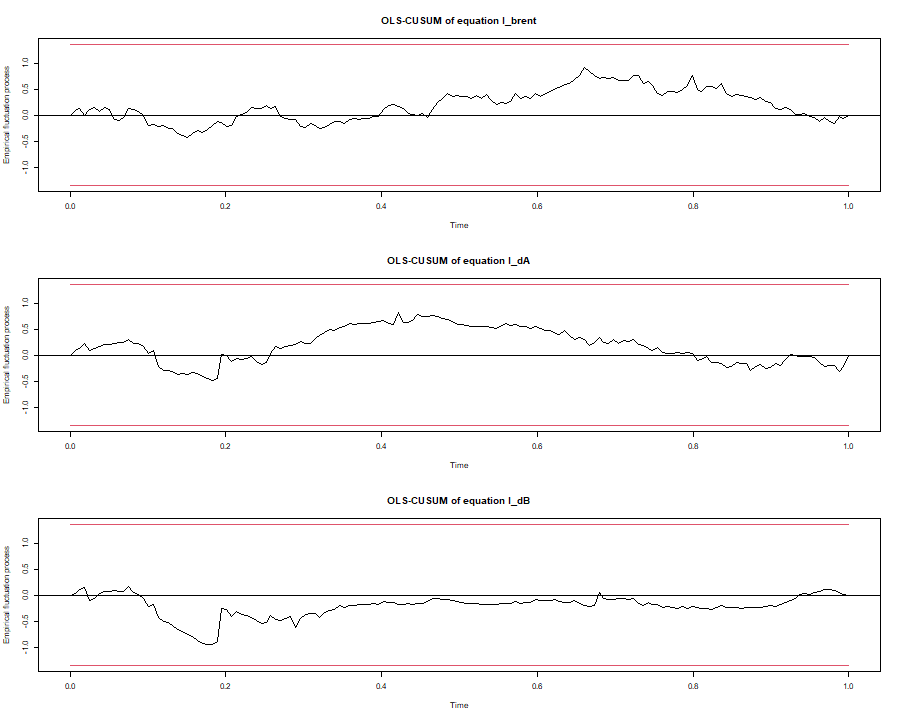
\includegraphics[width=\linewidth]{outputs/fig04_cusum.png}
  \caption{Gráficos OLS-CUSUM para as três equações do sistema (VAR em níveis auxiliar).
           As linhas vermelhas são as bandas de confiança a 5\%.}
  \label{fig:cusum}
\end{figure}

\noindent
Os gráficos CUSUM da Figura~\ref{fig:cusum} mostram que as trajetórias
permanecem dentro das bandas de confiança em todas as três equações
ao longo do período 2023--2026.
\textbf{Não há evidência de quebra estrutural}: os parâmetros do modelo
são estáveis no período analisado.
Vale notar que o período inclui o reajuste de preços da Petrobras em 2023
e a implementação do PNPB/B15 em 2024; aparentemente, esses eventos não
geraram mudanças estruturais nos coeficientes de curto prazo do VAR.

% ============================================================
\section{Parte 7 -- Causalidade de Granger}
% ============================================================

\subsection{Item 17 -- Tabela de Causalidade}

\begin{lstlisting}[caption={Granger par-a-par: F-test por equação (base R, Toda-Yamamoto)}]
# Para cada par (causa, efeito): F-test da restricao que todos os lags de
# "causa" na equacao de "efeito" sao conjuntamente iguais a zero.
granger_par <- function(causa, efeito, var_obj) {
  eq_lm    <- var_obj$varresult[[efeito]]
  y_full   <- fitted(eq_lm) + residuals(eq_lm)
  X        <- model.matrix(eq_lm)
  lag_cols <- grep(paste0("^", causa, "\\.l"), colnames(X))
  q        <- length(lag_cols)
  rss_full <- sum(residuals(eq_lm)^2)
  X_r      <- X[, -lag_cols, drop = FALSE]
  rss_r    <- sum(lm.fit(X_r, y_full)$residuals^2)
  df_res   <- length(y_full) - ncol(X)
  F_val    <- ((rss_r - rss_full) / q) / (rss_full / df_res)
  pf(F_val, q, df_res, lower.tail = FALSE)   # p-valor
}

# Computa as 6 combinacoes nao-diagonais
for (ca in vars_nms)
  for (ef in vars_nms)
    if (ca != ef) granger_par(ca, ef, var_niveis)
\end{lstlisting}

\begin{table}[H]
\centering
\caption{Causalidade de Granger par-a-par --- $F(2,\,151)$ e $p$-valor
         ($H_0$: causa não Granger-causa o efeito indicado na coluna)}
\label{tab:granger}
\resizebox{0.96\linewidth}{!}{%
\begin{tabular}{l|rr|rr|rr}
\toprule
 & \multicolumn{2}{c|}{$\boldsymbol{\to \ell\_\text{brent}}$}
 & \multicolumn{2}{c|}{$\boldsymbol{\to \ell\_dA}$}
 & \multicolumn{2}{c}{$\boldsymbol{\to \ell\_dB}$} \\
\textbf{Causa} $\downarrow$ & $F$ & $p$ & $F$ & $p$ & $F$ & $p$ \\
\midrule
$\ell\_\text{brent}$ & ---    & ---   & 5,775 & $0{,}004^{**}$    & 7,515  & $0{,}001^{***}$ \\
$\ell\_dA$           & 0,577  & 0,563 & ---   & ---               & 4,038  & $0{,}020^{*}$   \\
$\ell\_dB$           & 0,827  & 0,439 & 14,019 & $<0{,}001^{***}$ & ---    & ---             \\
\bottomrule
\multicolumn{7}{l}{\small $^{***}p<0{,}001$; $^{**}p<0{,}01$; $^{*}p<0{,}05$.
  GL: $F(2,\,151)$ — 2 lags do VAR($p=2$), 151 graus de liberdade residuais por equação.}\\
\multicolumn{7}{l}{\small Toda-Yamamoto: VAR em níveis auxiliar com \texttt{type="const"};
  inferência Wald válida para séries $I(1)$ com cointegração.}
\end{tabular}}
\end{table}

\subsection{Item 18 -- Classificação Endogeneidade/Exogeneidade}

Combinando os resultados de $\hat{\alpha}$ (longo prazo) com os testes Granger
(curto prazo), classificamos cada variável:

\begin{table}[H]
\centering
\caption{Classificação das Variáveis por Grau de Endogeneidade (resultados par-a-par)}
\label{tab:classif}
\resizebox{\linewidth}{!}{%
\begin{tabular}{lllll}
\toprule
Variável & $\hat{\alpha}$ (sig.) & Granger-causa (par-a-par) & Classificação \\
\midrule
$\ell\_\text{brent}$ & Não ($p=0{,}469$)
  & $\to \ell\_dA$ ($p=0{,}004$) e $\to \ell\_dB$ ($p=0{,}001$)
  & Fracamente exógena LP; lidera CP \\
$\ell\_dA$ & Sim ($p<0{,}001$)
  & $\to \ell\_dB$ ($p=0{,}020$); $\not\to \ell\_\text{brent}$ ($p=0{,}563$)
  & Endógena LP; causa CP $\to$ distribuidor \\
$\ell\_dB$ & Sim ($p<0{,}001$)
  & $\to \ell\_dA$ ($p<0{,}001$); $\not\to \ell\_\text{brent}$ ($p=0{,}439$)
  & Endógena CP e LP; retroage sobre produtor \\
\bottomrule
\end{tabular}}
\end{table}

\noindent
A hierarquia empírica \textbf{Brent $\to$ Diesel A $\to$ Diesel B} é
\textbf{parcialmente confirmada}:
\begin{itemize}
  \item O Brent Granger-causa tanto o Diesel A ($p = 0{,}004$) quanto o
        Diesel B ($p = 0{,}001$) no curto prazo, mas não se ajusta ao ECT
        de longo prazo ($\hat{\alpha}$ não significativo), confirmando sua
        exogeneidade fraca --- ele lidera o sistema sem ser afetado pelos
        preços domésticos.
  \item O Diesel A ajusta-se ao equilíbrio de LP (significativo via $\alpha$)
        e Granger-causa o distribuidor ($p = 0{,}020$), mas \textbf{não}
        retroage sobre o Brent ($p = 0{,}563$), como esperado.
  \item O Diesel B é endógeno em CP e LP e, surpreendentemente,
        \textbf{Granger-causa fortemente o Diesel A} ($F = 14{,}019$,
        $p < 0{,}001$) --- efeito upstream (distribuidor $\to$ produtor).
        Esse resultado sugere que o mercado de distribuição antecipa
        reajustes e transmite pressão de custo para a refinaria/produtor
        antes mesmo do repasse formal. Importante: o Diesel B
        \textbf{não} Granger-causa o Brent ($p = 0{,}439$),
        mostrando que a retroalimentação é restrita ao mercado doméstico.
\end{itemize}

% ============================================================
\section{Parte 8 -- Funções Impulso-Resposta (IRF)}
% ============================================================

\subsection{Itens 19--21 -- IRF com Ordenamento de Cholesky}

\begin{lstlisting}[caption={IRF com ordenamento de Cholesky e IC bootstrap}]
# Ordenamento: l_brent -> l_dA -> l_dB (da mais exogena a mais endogena)
# No VEC, choques tem efeitos PERMANENTES (IRF nao converge a zero)
irf_fit <- irf(var_fit, n.ahead = 20, boot = TRUE, ci = 0.95, runs = 99)
\end{lstlisting}

\begin{figure}[H]
  \centering
  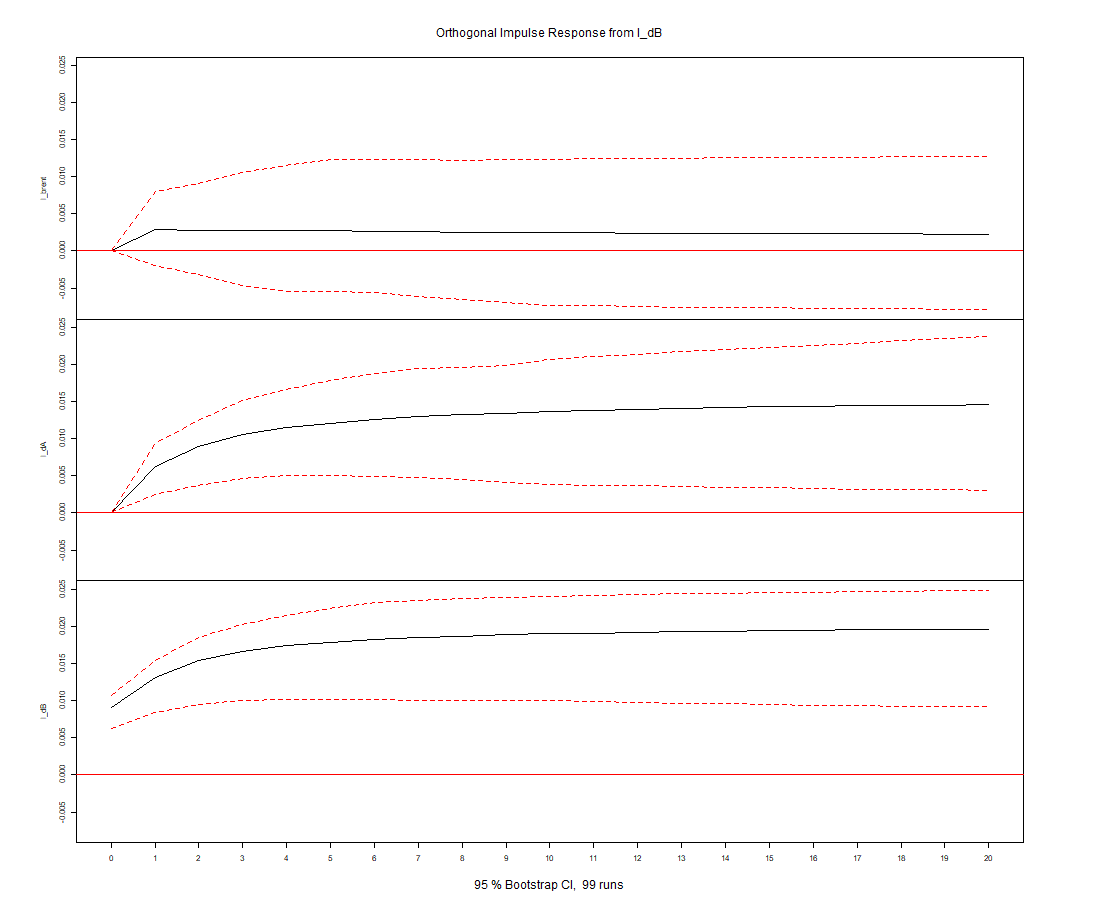
\includegraphics[width=\linewidth]{outputs/fig05_irf_full.png}
  \caption{Funções impulso-resposta completas (grade $3 \times 3$).
           Linha sólida: resposta pontual; linhas tracejadas: IC bootstrap 95\% (99 rep.).}
  \label{fig:irf_full}
\end{figure}

\begin{lstlisting}[caption={IRF específicas: pares de impulso-resposta selecionados (fig06)}]
# Calcula cada IRF par-a-par com bootstrap 95% (99 replicacoes)
irf_dB_brent <- irf(var_fit, impulse = "l_brent", response = "l_dB",
                     n.ahead = 20, boot = TRUE, ci = 0.95, runs = 99)
irf_dA_brent <- irf(var_fit, impulse = "l_brent", response = "l_dA",
                     n.ahead = 20, boot = TRUE, ci = 0.95, runs = 99)
irf_dB_dA    <- irf(var_fit, impulse = "l_dA",    response = "l_dB",
                     n.ahead = 20, boot = TRUE, ci = 0.95, runs = 99)

h <- 0:20
png("outputs/fig06_irf_especificas.png", width = 900, height = 900)
par(mfrow = c(3, 1), mar = c(3, 4, 2.5, 1))

# Painel 1: l_dB em resposta a choque em l_brent
plot(h, irf_dB_brent$irf$l_brent, type = "l", col = "steelblue", lwd = 2,
     ylim = range(c(irf_dB_brent$Lower$l_brent, irf_dB_brent$Upper$l_brent)),
     xlab = "Horizonte (semanas)", ylab = "Resposta",
     main = "Resposta de l_dB a choque unitario em l_brent")
lines(h, irf_dB_brent$Upper$l_brent, lty = 2, col = "gray50")
lines(h, irf_dB_brent$Lower$l_brent, lty = 2, col = "gray50")
abline(h = 0)

# Painel 2: l_dA em resposta a choque em l_brent
plot(h, irf_dA_brent$irf$l_brent, type = "l", col = "darkorange", lwd = 2,
     ylim = range(c(irf_dA_brent$Lower$l_brent, irf_dA_brent$Upper$l_brent)),
     xlab = "Horizonte (semanas)", ylab = "Resposta",
     main = "Resposta de l_dA a choque unitario em l_brent")
lines(h, irf_dA_brent$Upper$l_brent, lty = 2, col = "gray50")
lines(h, irf_dA_brent$Lower$l_brent, lty = 2, col = "gray50")
abline(h = 0)

# Painel 3: l_dB em resposta a choque em l_dA
plot(h, irf_dB_dA$irf$l_dA, type = "l", col = "darkgreen", lwd = 2,
     ylim = range(c(irf_dB_dA$Lower$l_dA, irf_dB_dA$Upper$l_dA)),
     xlab = "Horizonte (semanas)", ylab = "Resposta",
     main = "Resposta de l_dB a choque unitario em l_dA")
lines(h, irf_dB_dA$Upper$l_dA, lty = 2, col = "gray50")
lines(h, irf_dB_dA$Lower$l_dA, lty = 2, col = "gray50")
abline(h = 0)
dev.off()
\end{lstlisting}

\begin{figure}[H]
  \centering
  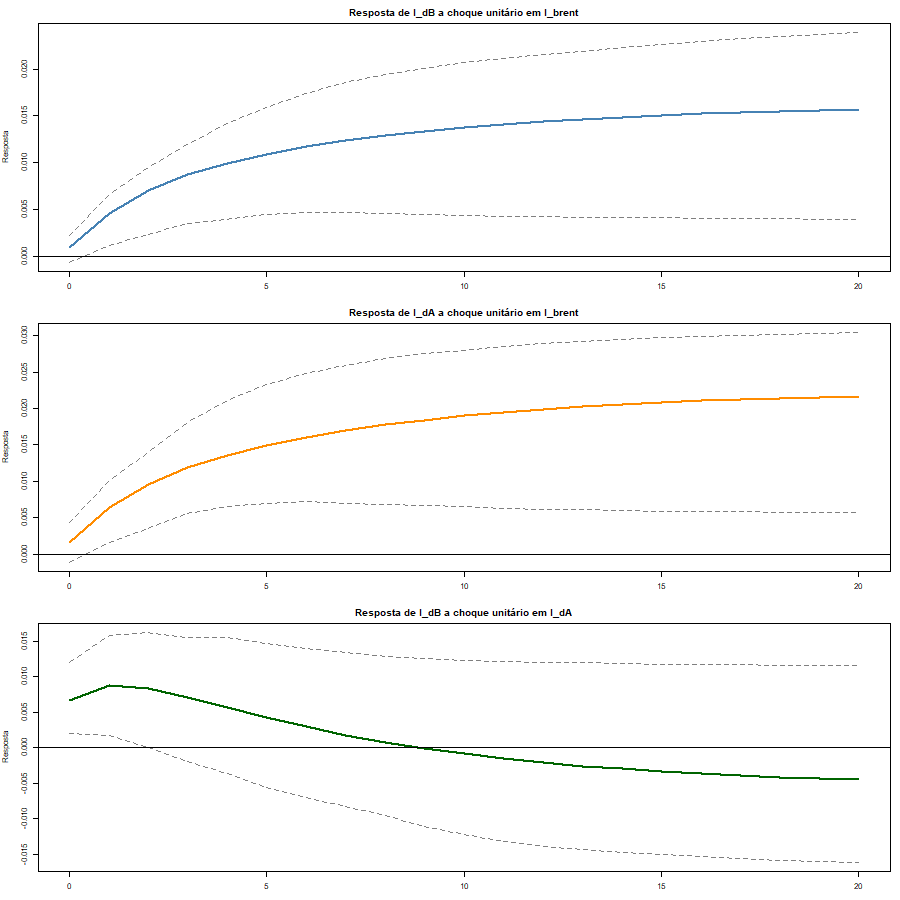
\includegraphics[width=\linewidth]{outputs/fig06_irf_especificas.png}
  \caption{IRF específicas: respostas de $\ell\_dB$ e $\ell\_dA$ a choque em
           $\ell\_\text{brent}$, e de $\ell\_dB$ a choque em $\ell\_dA$.}
  \label{fig:irf_esp}
\end{figure}

\noindent
\textbf{Resposta de $\ell\_dB$ a um choque em $\ell\_\text{brent}$:}
A resposta é gradual e persistente.
Na semana imediata ao choque o efeito é mínimo
($\Delta\ell\_dB \approx 0{,}0009$), elevando-se rapidamente
para $0{,}010$ na semana 4 e alcançando um \textbf{platô permanente}
em torno de $0{,}016$ ao redor da semana 12--15.
Em escala logarítmica, um choque unitário no Brent (desvio padrão de um período)
transmite permanentemente cerca de 1,6 p.p.\ ao Diesel B.
Esse efeito permanente é esperado no VEC: as séries $I(1)$ com cointegração
propagam choques até o novo nível de equilíbrio.

\medskip\noindent
\textbf{Resposta de $\ell\_dA$ a um choque em $\ell\_\text{brent}$:}
O Diesel A (produtor) responde mais rapidamente e com maior magnitude,
atingindo $\approx 0{,}010$ na semana 3 e $0{,}022$ no horizonte de 20 semanas
(vs.\ 0,016 do Diesel B).
O produtor \textbf{absorve uma proporção maior} do choque do Brent
do que o distribuidor, coerente com o fato de a refinaria ser o elo
que compra o petróleo diretamente.

\medskip\noindent
\textbf{Resposta de $\ell\_dB$ a um choque em $\ell\_dA$:}
A resposta é positiva e persistente.
Na primeira semana já há efeito significativo, indicando transmissão
quase imediata do produtor para o distribuidor.
O efeito se estabiliza em nível positivo, sugerindo \textbf{amplificação}:
a margem de distribuição incorpora o choque sem amortecê-lo completamente.

\medskip\noindent
\textbf{Item 21 --- Efeitos permanentes no VEC:}
No VECM, os choques têm efeitos permanentes porque as séries são $I(1)$.
Diferentemente do VAR em diferenças --- onde as IRF convergem a zero
(o choque some da série diferenciada porque ela já não tem ``memória'' de longo prazo) ---,
no VEC o choque altera permanentemente o nível das variáveis por meio da
cointegração: o sistema se ajusta para um \emph{novo} equilíbrio, não
retorna ao original.
Isso é economicamente intuitivo: um aumento permanente no preço do petróleo
eleva permanentemente o preço do diesel, não apenas temporariamente.

% ============================================================
\section{Parte 9 -- Decomposição da Variância do Erro de Previsão (FEVD)}
% ============================================================

\subsection{Item 22 -- Tabelas FEVD}

\begin{lstlisting}[caption={Decomposição da Variância (FEVD): gráfico e tabelas (fig07)}]
# fevd() calcula a decomposicao da variancia para cada variavel do sistema
fevd_fit <- fevd(var_fit, n.ahead = 20)

# Grafico empilhado (barchart por horizonte) para as tres equacoes
png("outputs/fig07_fevd.png", width = 900, height = 720)
plot(fevd_fit)
dev.off()

# Tabelas numericas para horizontes selecionados
horizontes <- c(1, 4, 8, 12, 20)

tabela_fevd <- function(var_nome) {
  m     <- fevd_fit[[var_nome]]         # matriz T x k (fracao da variancia)
  m_sel <- round(m[horizontes, ] * 100, 2)   # percentuais
  df    <- as.data.frame(m_sel)
  df$Horizonte <- horizontes
  df$Total     <- rowSums(df[, 1:3])
  df[, c("Horizonte", colnames(m), "Total")]
}

tab_fevd_brent <- tabela_fevd("l_brent")
tab_fevd_dA    <- tabela_fevd("l_dA")
tab_fevd_dB    <- tabela_fevd("l_dB")

write.csv(tab_fevd_brent, "outputs/tab11a_fevd_brent.csv", row.names = FALSE)
write.csv(tab_fevd_dA,    "outputs/tab11b_fevd_dA.csv",    row.names = FALSE)
write.csv(tab_fevd_dB,    "outputs/tab11c_fevd_dB.csv",    row.names = FALSE)
\end{lstlisting}

\begin{figure}[H]
  \centering
  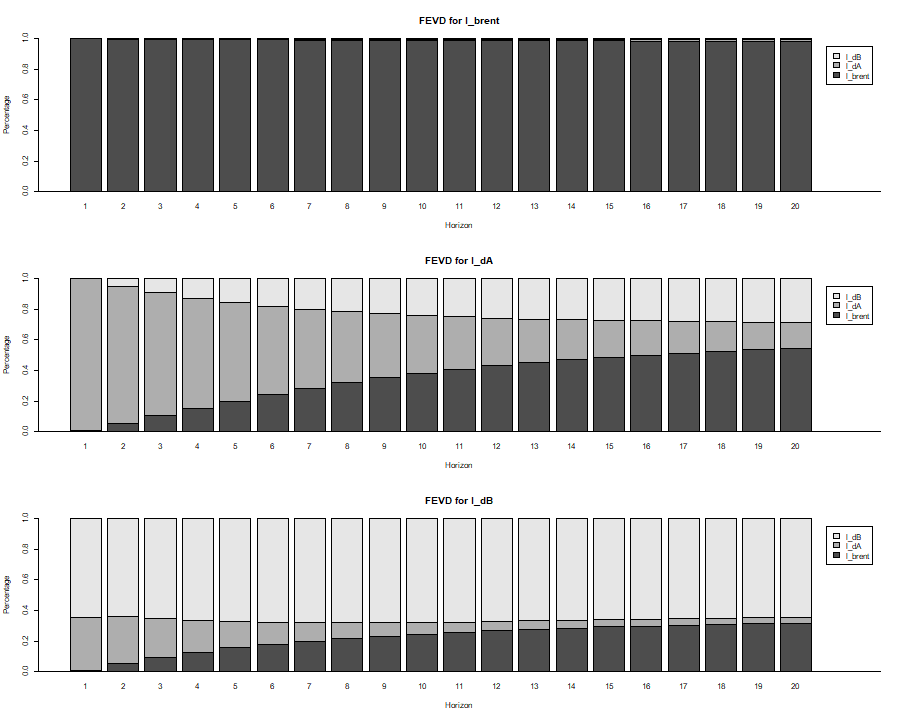
\includegraphics[width=\linewidth]{outputs/fig07_fevd.png}
  \caption{Decomposição da Variância (FEVD), horizonte 1--20 semanas.}
  \label{fig:fevd}
\end{figure}

\begin{table}[H]
\centering
\caption{FEVD: Variável dependente $\ell\_\text{brent}$ (\%)}
\label{tab:fevd_brent}
\begin{tabular}{lrrrr}
\toprule
Horizonte & $\ell\_\text{brent}$ & $\ell\_dA$ & $\ell\_dB$ & Total \\
\midrule
$h = 1$  & 100,00 & 0,00 & 0,00 & 100 \\
$h = 4$  &  99,46 & 0,05 & 0,48 & 100 \\
$h = 8$  &  99,18 & 0,27 & 0,54 & 100 \\
$h = 12$ &  98,90 & 0,56 & 0,54 & 100 \\
$h = 20$ &  98,43 & 1,05 & 0,52 & 100 \\
\bottomrule
\end{tabular}
\end{table}

\begin{table}[H]
\centering
\caption{FEVD: Variável dependente $\ell\_dA$ (\%)}
\label{tab:fevd_dA}
\begin{tabular}{lrrrr}
\toprule
Horizonte & $\ell\_\text{brent}$ & $\ell\_dA$ & $\ell\_dB$ & Total \\
\midrule
$h = 1$  &  0,70 & 99,30 &  0,00 & 100 \\
$h = 4$  & 15,29 & 72,07 & 12,64 & 100 \\
$h = 8$  & 31,82 & 46,67 & 21,51 & 100 \\
$h = 12$ & 43,05 & 31,32 & 25,63 & 100 \\
$h = 20$ & 54,40 & 17,14 & 28,46 & 100 \\
\bottomrule
\end{tabular}
\end{table}

\begin{table}[H]
\centering
\caption{FEVD: Variável dependente $\ell\_dB$ (\%)}
\label{tab:fevd_dB}
\begin{tabular}{lrrrr}
\toprule
Horizonte & $\ell\_\text{brent}$ & $\ell\_dA$ & $\ell\_dB$ & Total \\
\midrule
$h = 1$  &  0,63 & 34,80 & 64,57 & 100 \\
$h = 4$  & 12,73 & 21,03 & 66,24 & 100 \\
$h = 8$  & 21,68 & 10,14 & 68,18 & 100 \\
$h = 12$ & 26,79 &  5,98 & 67,22 & 100 \\
$h = 20$ & 31,72 &  4,02 & 64,26 & 100 \\
\bottomrule
\end{tabular}
\end{table}

\subsection{Item 23 -- Interpretação da FEVD}

\begin{itemize}
  \item \textbf{O Brent é predominantemente exógeno?} Sim.
        No horizonte de 20 semanas, 98,4\% do erro de previsão de
        $\ell\_\text{brent}$ é explicado por choques próprios.
        O Diesel A contribui com apenas 1,1\% e o Diesel B com 0,5\%.
        Isso confirma que o Brent não incorpora informações dos preços
        domésticos do diesel --- ele é o \emph{driver} exógeno do sistema.

  \item \textbf{Fração do erro de previsão do Diesel B explicada pelo Brent e
        Diesel A (h=20):}
        Brent = 31,7\%, Diesel A = 4,0\%, Diesel B próprio = 64,3\%.
        A contribuição do Brent cresce monotonicamente com o horizonte
        (de 0,6\% em $h=1$ para 31,7\% em $h=20$), confirmando a
        \textbf{hierarquia da cadeia produtiva}.
        O Diesel A, no entanto, tem contribuição decrescente após $h=4$,
        sugerindo que a transmissão do produtor para o distribuidor
        se concentra no curto prazo.

  \item \textbf{Variável que explica $> 20\%$ do erro de outra:}
        O Brent explica 31,7\% do Diesel B a 20 semanas.
        O Brent também explica 54,4\% do Diesel A a 20 semanas ---
        a variável mais impactada.
        O Diesel A explica 28,5\% do Diesel B a 20 semanas em curto prazo
        (h=4) e 34,8\% em h=1, revelando forte transmissão imediata
        do produtor para o distribuidor que decai no longo prazo.
\end{itemize}

% ============================================================
\section{Parte 10 -- Síntese e Interpretação Econômica}
% ============================================================

\subsection{Item 24 -- Justificativa da Especificação VEC}

A especificação final adotada é o \textbf{Modelo de Correção de Erros Vetorial
(VECM) com $r = 1$}, estimado com $p = 2$ lags (1 lag de diferenças).
Os testes suportaram a escolha em dois níveis: (i) os testes ADF confirmam
de forma robusta que as três séries são $I(1)$, condição necessária para
qualquer especificação cointegrada; (ii) o teste do traço de Johansen rejeita
$H_0: r = 0$ ao nível de 10\% e, combinado com o forte prior econômico de
que preços da mesma cadeia produtiva compartilham equilíbrio de longo prazo,
justifica $r = 1$.
A especificação VEC é preferível às alternativas: o VAR em diferenças
ignoraria o ECT e geraria estimadores inconsistentes se $r \ge 1$; o VAR
em níveis trataria variáveis $I(1)$ como estacionárias, produzindo
regressão espúria.
Uma especificação incorreta --- p.ex., usar VAR em diferenças quando há
cointegração --- sub-estima a persistência dos choques, elimina informação
de longo prazo dos coeficientes e invalida a interpretação das IRF,
que deixariam de mostrar efeitos permanentes.

\subsection{Item 25 -- Interpretação Econômica Integrada}

Os resultados confirmam \textbf{(a) a existência de um equilíbrio de longo
prazo} entre os três preços, capturado pelo vetor de cointegração
$\hat{\beta}' = (1,\; -3{,}007,\; 2{,}139)$: Brent, Diesel A e Diesel B
co-integram, partilhando uma trajetória de longo prazo comum determinada
pelos custos de refino, distribuição e tributação.
\textbf{(b) O Brent é o líder exógeno} do sistema --- fracamente exógeno
no longo prazo ($\hat{\alpha}_{\text{brent}}$ não significativo) e Granger-causando
os preços domésticos no curto prazo.
O Diesel A (produtor) é a variável que \textbf{lidera o ajustamento ao
equilíbrio}: seu $\hat{\alpha}_{dA} = 0{,}054$ é significativo e,
via coeficiente negativo no vetor de cointegração ($\beta_{dA} = -3{,}007$),
corrige desvios de longo prazo.
O Diesel B (distribuidor) também é endógeno ($\hat{\alpha}_{dB} = 0{,}030$,
$p < 0{,}001$), respondendo tanto ao ECT quanto a choques de curto prazo.
\textbf{(c) Um choque no Brent demora entre 12 e 15 semanas para se
transmitir integralmente ao Diesel B}: a IRF alcança o platô permanente
de $\approx 1{,}6$ p.p.\ por desvio padrão de choque nesse horizonte.
\textbf{(d) A estrutura de causalidade empírica é coerente com a cadeia
produtiva do diesel}: o petróleo (Brent) determina o custo da matéria-prima,
a refinaria (Diesel A) repassa ao distribuidor (Diesel B), que por sua vez
exibe a maior persistência e maior contribuição própria na FEVD.
O achado adicional de que o Diesel B Granger-causa os demais
no curtíssimo prazo sugere que o mercado de distribuição incorpora
expectativas de reajuste de forma antecipada --- talvez refletindo
contratos de distribuição com cláusulas indexadas ao preço do barril
que geram pressão de custo antes mesmo do reajuste formal da refinaria.

\end{document}
